\documentclass[class=minimal,border=0pt]{standalone}
\usepackage{hyperref}
\hypersetup{
colorlinks=true,
urlcolor=cyan}
\usepackage{tikz}
\begin{document}
%\documentclass{standalone}
%\usepackage{tikz}
%\usetikzlibrary{patterns,plotmarks}
%\begin{document}
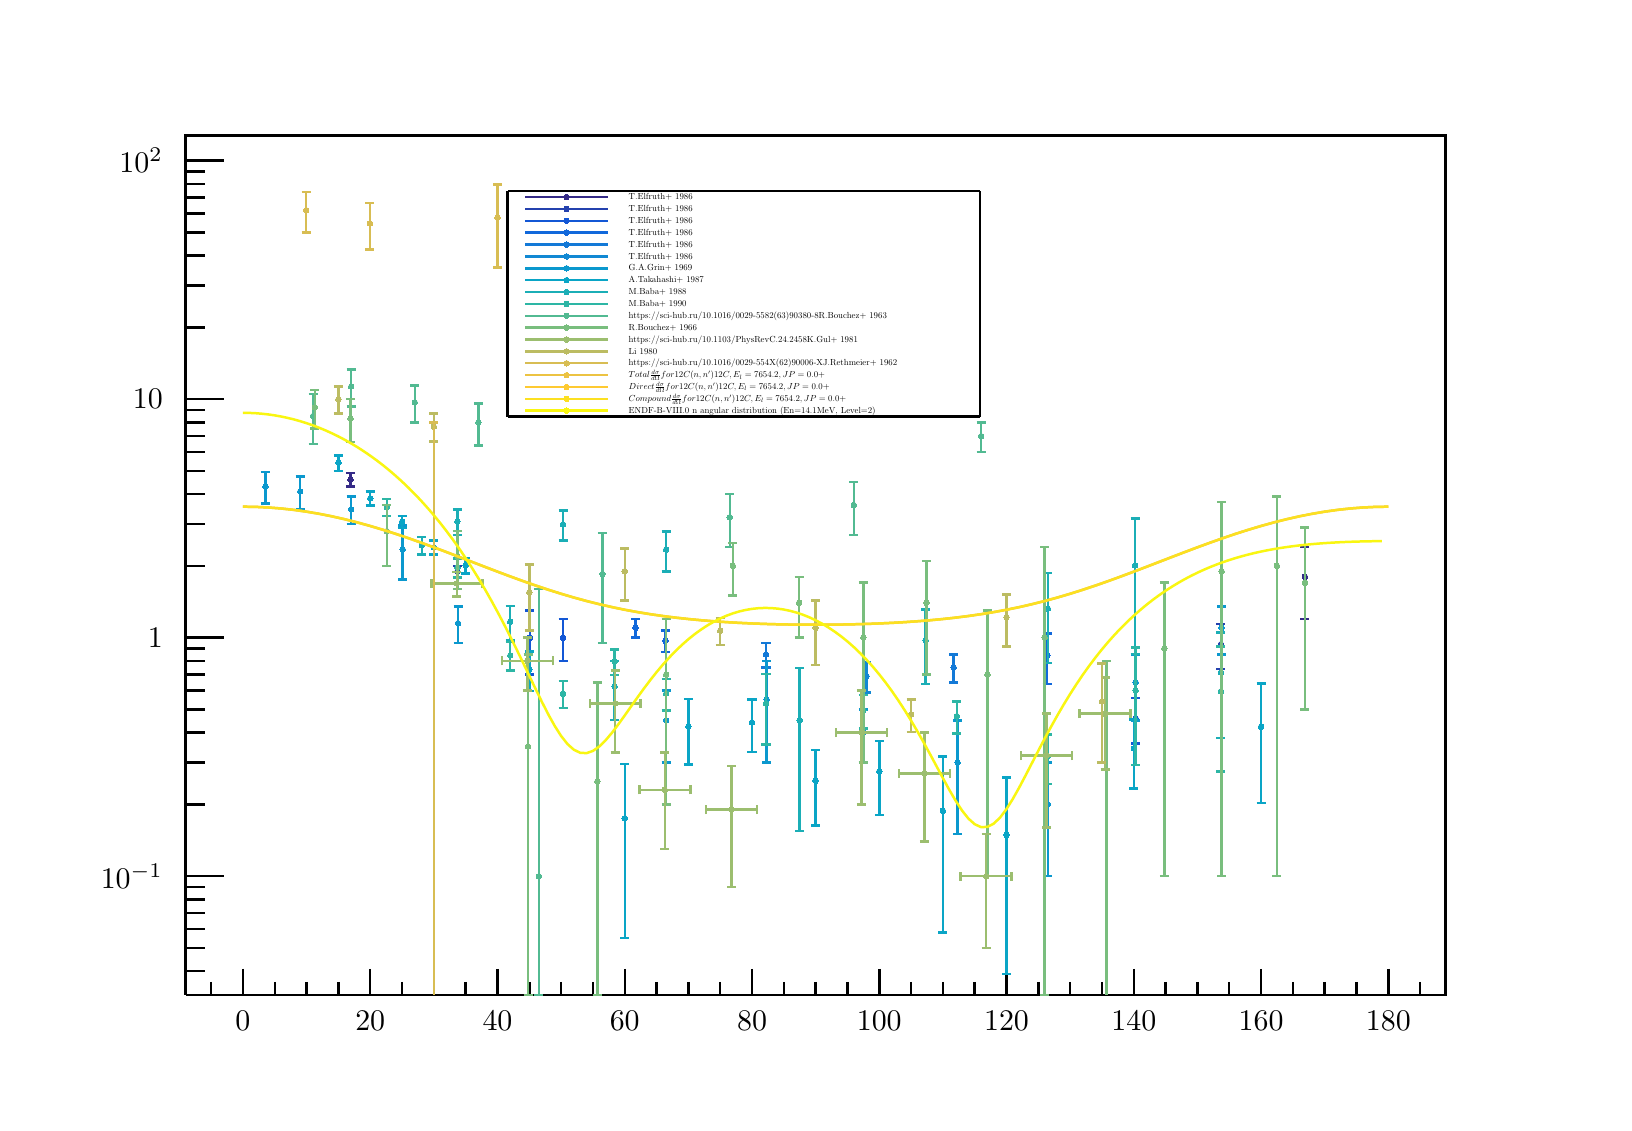
\begin{tikzpicture}
\def\CheckTikzLibraryLoaded#1{ \ifcsname tikz@library@#1@loaded\endcsname \else \PackageWarning{tikz}{usetikzlibrary{#1} is missing in the preamble.} \fi }
\CheckTikzLibraryLoaded{patterns}
\CheckTikzLibraryLoaded{plotmarks}
\pgfdeclareplotmark{cross} {
\pgfpathmoveto{\pgfpoint{-0.3\pgfplotmarksize}{\pgfplotmarksize}}
\pgfpathlineto{\pgfpoint{+0.3\pgfplotmarksize}{\pgfplotmarksize}}
\pgfpathlineto{\pgfpoint{+0.3\pgfplotmarksize}{0.3\pgfplotmarksize}}
\pgfpathlineto{\pgfpoint{+1\pgfplotmarksize}{0.3\pgfplotmarksize}}
\pgfpathlineto{\pgfpoint{+1\pgfplotmarksize}{-0.3\pgfplotmarksize}}
\pgfpathlineto{\pgfpoint{+0.3\pgfplotmarksize}{-0.3\pgfplotmarksize}}
\pgfpathlineto{\pgfpoint{+0.3\pgfplotmarksize}{-1.\pgfplotmarksize}}
\pgfpathlineto{\pgfpoint{-0.3\pgfplotmarksize}{-1.\pgfplotmarksize}}
\pgfpathlineto{\pgfpoint{-0.3\pgfplotmarksize}{-0.3\pgfplotmarksize}}
\pgfpathlineto{\pgfpoint{-1.\pgfplotmarksize}{-0.3\pgfplotmarksize}}
\pgfpathlineto{\pgfpoint{-1.\pgfplotmarksize}{0.3\pgfplotmarksize}}
\pgfpathlineto{\pgfpoint{-0.3\pgfplotmarksize}{0.3\pgfplotmarksize}}
\pgfpathclose
\pgfusepathqstroke
}
\pgfdeclareplotmark{cross*} {
\pgfpathmoveto{\pgfpoint{-0.3\pgfplotmarksize}{\pgfplotmarksize}}
\pgfpathlineto{\pgfpoint{+0.3\pgfplotmarksize}{\pgfplotmarksize}}
\pgfpathlineto{\pgfpoint{+0.3\pgfplotmarksize}{0.3\pgfplotmarksize}}
\pgfpathlineto{\pgfpoint{+1\pgfplotmarksize}{0.3\pgfplotmarksize}}
\pgfpathlineto{\pgfpoint{+1\pgfplotmarksize}{-0.3\pgfplotmarksize}}
\pgfpathlineto{\pgfpoint{+0.3\pgfplotmarksize}{-0.3\pgfplotmarksize}}
\pgfpathlineto{\pgfpoint{+0.3\pgfplotmarksize}{-1.\pgfplotmarksize}}
\pgfpathlineto{\pgfpoint{-0.3\pgfplotmarksize}{-1.\pgfplotmarksize}}
\pgfpathlineto{\pgfpoint{-0.3\pgfplotmarksize}{-0.3\pgfplotmarksize}}
\pgfpathlineto{\pgfpoint{-1.\pgfplotmarksize}{-0.3\pgfplotmarksize}}
\pgfpathlineto{\pgfpoint{-1.\pgfplotmarksize}{0.3\pgfplotmarksize}}
\pgfpathlineto{\pgfpoint{-0.3\pgfplotmarksize}{0.3\pgfplotmarksize}}
\pgfpathclose
\pgfusepathqfillstroke
}
\pgfdeclareplotmark{newstar} {
\pgfpathmoveto{\pgfqpoint{0pt}{\pgfplotmarksize}}
\pgfpathlineto{\pgfqpointpolar{44}{0.5\pgfplotmarksize}}
\pgfpathlineto{\pgfqpointpolar{18}{\pgfplotmarksize}}
\pgfpathlineto{\pgfqpointpolar{-20}{0.5\pgfplotmarksize}}
\pgfpathlineto{\pgfqpointpolar{-54}{\pgfplotmarksize}}
\pgfpathlineto{\pgfqpointpolar{-90}{0.5\pgfplotmarksize}}
\pgfpathlineto{\pgfqpointpolar{234}{\pgfplotmarksize}}
\pgfpathlineto{\pgfqpointpolar{198}{0.5\pgfplotmarksize}}
\pgfpathlineto{\pgfqpointpolar{162}{\pgfplotmarksize}}
\pgfpathlineto{\pgfqpointpolar{134}{0.5\pgfplotmarksize}}
\pgfpathclose
\pgfusepathqstroke
}
\pgfdeclareplotmark{newstar*} {
\pgfpathmoveto{\pgfqpoint{0pt}{\pgfplotmarksize}}
\pgfpathlineto{\pgfqpointpolar{44}{0.5\pgfplotmarksize}}
\pgfpathlineto{\pgfqpointpolar{18}{\pgfplotmarksize}}
\pgfpathlineto{\pgfqpointpolar{-20}{0.5\pgfplotmarksize}}
\pgfpathlineto{\pgfqpointpolar{-54}{\pgfplotmarksize}}
\pgfpathlineto{\pgfqpointpolar{-90}{0.5\pgfplotmarksize}}
\pgfpathlineto{\pgfqpointpolar{234}{\pgfplotmarksize}}
\pgfpathlineto{\pgfqpointpolar{198}{0.5\pgfplotmarksize}}
\pgfpathlineto{\pgfqpointpolar{162}{\pgfplotmarksize}}
\pgfpathlineto{\pgfqpointpolar{134}{0.5\pgfplotmarksize}}
\pgfpathclose
\pgfusepathqfillstroke
}
\definecolor{c}{rgb}{1,1,1};
\draw [color=c, fill=c] (0,0) rectangle (20,13.639);
\draw [color=c, fill=c] (2,1.3639) rectangle (18,12.2751);
\definecolor{c}{rgb}{0,0,0};
\draw [c,line width=0.9] (2,1.3639) -- (2,12.2751) -- (18,12.2751) -- (18,1.3639) -- (2,1.3639);
\draw [c,line width=0.9] (2,1.3639) -- (18,1.3639);
\draw [c,line width=0.9] (2.72727,1.69123) -- (2.72727,1.3639);
\draw [c,line width=0.9] (3.13131,1.52756) -- (3.13131,1.3639);
\draw [c,line width=0.9] (3.53535,1.52756) -- (3.53535,1.3639);
\draw [c,line width=0.9] (3.93939,1.52756) -- (3.93939,1.3639);
\draw [c,line width=0.9] (4.34343,1.69123) -- (4.34343,1.3639);
\draw [c,line width=0.9] (4.74747,1.52756) -- (4.74747,1.3639);
\draw [c,line width=0.9] (5.15152,1.52756) -- (5.15152,1.3639);
\draw [c,line width=0.9] (5.55556,1.52756) -- (5.55556,1.3639);
\draw [c,line width=0.9] (5.9596,1.69123) -- (5.9596,1.3639);
\draw [c,line width=0.9] (6.36364,1.52756) -- (6.36364,1.3639);
\draw [c,line width=0.9] (6.76768,1.52756) -- (6.76768,1.3639);
\draw [c,line width=0.9] (7.17172,1.52756) -- (7.17172,1.3639);
\draw [c,line width=0.9] (7.57576,1.69123) -- (7.57576,1.3639);
\draw [c,line width=0.9] (7.9798,1.52756) -- (7.9798,1.3639);
\draw [c,line width=0.9] (8.38384,1.52756) -- (8.38384,1.3639);
\draw [c,line width=0.9] (8.78788,1.52756) -- (8.78788,1.3639);
\draw [c,line width=0.9] (9.19192,1.69123) -- (9.19192,1.3639);
\draw [c,line width=0.9] (9.59596,1.52756) -- (9.59596,1.3639);
\draw [c,line width=0.9] (10,1.52756) -- (10,1.3639);
\draw [c,line width=0.9] (10.404,1.52756) -- (10.404,1.3639);
\draw [c,line width=0.9] (10.8081,1.69123) -- (10.8081,1.3639);
\draw [c,line width=0.9] (11.2121,1.52756) -- (11.2121,1.3639);
\draw [c,line width=0.9] (11.6162,1.52756) -- (11.6162,1.3639);
\draw [c,line width=0.9] (12.0202,1.52756) -- (12.0202,1.3639);
\draw [c,line width=0.9] (12.4242,1.69123) -- (12.4242,1.3639);
\draw [c,line width=0.9] (12.8283,1.52756) -- (12.8283,1.3639);
\draw [c,line width=0.9] (13.2323,1.52756) -- (13.2323,1.3639);
\draw [c,line width=0.9] (13.6364,1.52756) -- (13.6364,1.3639);
\draw [c,line width=0.9] (14.0404,1.69123) -- (14.0404,1.3639);
\draw [c,line width=0.9] (14.4444,1.52756) -- (14.4444,1.3639);
\draw [c,line width=0.9] (14.8485,1.52756) -- (14.8485,1.3639);
\draw [c,line width=0.9] (15.2525,1.52756) -- (15.2525,1.3639);
\draw [c,line width=0.9] (15.6566,1.69123) -- (15.6566,1.3639);
\draw [c,line width=0.9] (16.0606,1.52756) -- (16.0606,1.3639);
\draw [c,line width=0.9] (16.4646,1.52756) -- (16.4646,1.3639);
\draw [c,line width=0.9] (16.8687,1.52756) -- (16.8687,1.3639);
\draw [c,line width=0.9] (17.2727,1.69123) -- (17.2727,1.3639);
\draw [c,line width=0.9] (2.72727,1.69123) -- (2.72727,1.3639);
\draw [c,line width=0.9] (2.32323,1.52756) -- (2.32323,1.3639);
\draw [c,line width=0.9] (17.2727,1.69123) -- (17.2727,1.3639);
\draw [c,line width=0.9] (17.6768,1.52756) -- (17.6768,1.3639);
\draw [anchor=base] (2.72727,0.913811) node[scale=1.08185, color=c, rotate=0]{0};
\draw [anchor=base] (4.34343,0.913811) node[scale=1.08185, color=c, rotate=0]{20};
\draw [anchor=base] (5.9596,0.913811) node[scale=1.08185, color=c, rotate=0]{40};
\draw [anchor=base] (7.57576,0.913811) node[scale=1.08185, color=c, rotate=0]{60};
\draw [anchor=base] (9.19192,0.913811) node[scale=1.08185, color=c, rotate=0]{80};
\draw [anchor=base] (10.8081,0.913811) node[scale=1.08185, color=c, rotate=0]{100};
\draw [anchor=base] (12.4242,0.913811) node[scale=1.08185, color=c, rotate=0]{120};
\draw [anchor=base] (14.0404,0.913811) node[scale=1.08185, color=c, rotate=0]{140};
\draw [anchor=base] (15.6566,0.913811) node[scale=1.08185, color=c, rotate=0]{160};
\draw [anchor=base] (17.2727,0.913811) node[scale=1.08185, color=c, rotate=0]{180};
\draw [c,line width=0.9] (2,1.3639) -- (2,12.2751);
\draw [c,line width=0.9] (2.24,1.66405) -- (2,1.66405);
\draw [c,line width=0.9] (2.24,1.9576) -- (2,1.9576);
\draw [c,line width=0.9] (2.24,2.19746) -- (2,2.19746);
\draw [c,line width=0.9] (2.24,2.40025) -- (2,2.40025);
\draw [c,line width=0.9] (2.24,2.57591) -- (2,2.57591);
\draw [c,line width=0.9] (2.24,2.73086) -- (2,2.73086);
\draw [c,line width=0.9] (2.48,2.86947) -- (2,2.86947);
\draw [anchor= east] (1.844,2.86947) node[scale=1.08185, color=c, rotate=0]{$10^{-1}$};
\draw [c,line width=0.9] (2.24,3.78133) -- (2,3.78133);
\draw [c,line width=0.9] (2.24,4.31474) -- (2,4.31474);
\draw [c,line width=0.9] (2.24,4.6932) -- (2,4.6932);
\draw [c,line width=0.9] (2.24,4.98675) -- (2,4.98675);
\draw [c,line width=0.9] (2.24,5.2266) -- (2,5.2266);
\draw [c,line width=0.9] (2.24,5.42939) -- (2,5.42939);
\draw [c,line width=0.9] (2.24,5.60506) -- (2,5.60506);
\draw [c,line width=0.9] (2.24,5.76001) -- (2,5.76001);
\draw [c,line width=0.9] (2.48,5.89862) -- (2,5.89862);
\draw [anchor= east] (1.844,5.89862) node[scale=1.08185, color=c, rotate=0]{1};
\draw [c,line width=0.9] (2.24,6.81048) -- (2,6.81048);
\draw [c,line width=0.9] (2.24,7.34389) -- (2,7.34389);
\draw [c,line width=0.9] (2.24,7.72234) -- (2,7.72234);
\draw [c,line width=0.9] (2.24,8.0159) -- (2,8.0159);
\draw [c,line width=0.9] (2.24,8.25575) -- (2,8.25575);
\draw [c,line width=0.9] (2.24,8.45854) -- (2,8.45854);
\draw [c,line width=0.9] (2.24,8.63421) -- (2,8.63421);
\draw [c,line width=0.9] (2.24,8.78916) -- (2,8.78916);
\draw [c,line width=0.9] (2.48,8.92776) -- (2,8.92776);
\draw [anchor= east] (1.844,8.92776) node[scale=1.08185, color=c, rotate=0]{10};
\draw [c,line width=0.9] (2.24,9.83963) -- (2,9.83963);
\draw [c,line width=0.9] (2.24,10.373) -- (2,10.373);
\draw [c,line width=0.9] (2.24,10.7515) -- (2,10.7515);
\draw [c,line width=0.9] (2.24,11.045) -- (2,11.045);
\draw [c,line width=0.9] (2.24,11.2849) -- (2,11.2849);
\draw [c,line width=0.9] (2.24,11.4877) -- (2,11.4877);
\draw [c,line width=0.9] (2.24,11.6634) -- (2,11.6634);
\draw [c,line width=0.9] (2.24,11.8183) -- (2,11.8183);
\draw [c,line width=0.9] (2.48,11.9569) -- (2,11.9569);
\draw [anchor= east] (1.844,11.9569) node[scale=1.08185, color=c, rotate=0]{$10^{2}$};
\definecolor{c}{rgb}{0.2082,0.1664,0.5293};
\draw [c,line width=0.9] (4.09294,7.90621) -- (4.09294,7.98932);
\draw [c,line width=0.9] (4.03563,7.98932) -- (4.15024,7.98932);
\draw [c,line width=0.9] (4.09294,7.90621) -- (4.09294,7.81748);
\draw [c,line width=0.9] (4.03563,7.81748) -- (4.15024,7.81748);
\draw [c,line width=0.9] (16.2141,6.67187) -- (16.2141,7.05033);
\draw [c,line width=0.9] (16.1568,7.05033) -- (16.2714,7.05033);
\draw [c,line width=0.9] (16.2141,6.67187) -- (16.2141,6.13847);
\draw [c,line width=0.9] (16.1568,6.13847) -- (16.2714,6.13847);
\foreach \P in {(4.09294,7.90621), (16.2141,6.67187)}{\draw[mark options={color=c,fill=c},mark size=2.402402pt, line width=0.000000pt, mark=*,mark size=1pt] plot coordinates {\P};}
\definecolor{c}{rgb}{0.14091,0.253787,0.682442};
\draw [c,line width=0.9] (5.4505,6.743) -- (5.4505,6.81048);
\draw [c,line width=0.9] (5.39319,6.81048) -- (5.50781,6.81048);
\draw [c,line width=0.9] (5.4505,6.743) -- (5.4505,6.67187);
\draw [c,line width=0.9] (5.39319,6.67187) -- (5.50781,6.67187);
\draw [c,line width=0.9] (15.1475,5.81721) -- (15.1475,6.07099);
\draw [c,line width=0.9] (15.0902,6.07099) -- (15.2048,6.07099);
\draw [c,line width=0.9] (15.1475,5.81721) -- (15.1475,5.5025);
\draw [c,line width=0.9] (15.0902,5.5025) -- (15.2048,5.5025);
\foreach \P in {(5.4505,6.743), (15.1475,5.81721)}{\draw[mark options={color=c,fill=c},mark size=2.402402pt, line width=0.000000pt, mark=*,mark size=1pt] plot coordinates {\P};}
\definecolor{c}{rgb}{0.0736194,0.341174,0.835584};
\draw [c,line width=0.9] (6.37171,5.89861) -- (6.37171,6.24377);
\draw [c,line width=0.9] (6.31441,6.24377) -- (6.42902,6.24377);
\draw [c,line width=0.9] (6.37171,5.89861) -- (6.37171,5.42939);
\draw [c,line width=0.9] (6.31441,5.42939) -- (6.42902,5.42939);
\draw [c,line width=0.9] (6.79191,5.89861) -- (6.79191,6.13847);
\draw [c,line width=0.9] (6.73461,6.13847) -- (6.84922,6.13847);
\draw [c,line width=0.9] (6.79191,5.89861) -- (6.79191,5.60506);
\draw [c,line width=0.9] (6.73461,5.60506) -- (6.84922,5.60506);
\draw [c,line width=0.9] (14.0646,4.87706) -- (14.0646,5.13584);
\draw [c,line width=0.9] (14.0073,5.13584) -- (14.1219,5.13584);
\draw [c,line width=0.9] (14.0646,4.87706) -- (14.0646,4.55459);
\draw [c,line width=0.9] (14.0073,4.55459) -- (14.1219,4.55459);
\foreach \P in {(6.37171,5.89861), (6.79191,5.89861), (14.0646,4.87706)}{\draw[mark options={color=c,fill=c},mark size=2.402402pt, line width=0.000000pt, mark=*,mark size=1pt] plot coordinates {\P};}
\definecolor{c}{rgb}{0.0656625,0.409469,0.858122};
\draw [c,line width=0.9] (7.71313,6.024) -- (7.71313,6.13847);
\draw [c,line width=0.9] (7.65582,6.13847) -- (7.77043,6.13847);
\draw [c,line width=0.9] (7.71313,6.024) -- (7.71313,5.89861);
\draw [c,line width=0.9] (7.65582,5.89861) -- (7.77043,5.89861);
\draw [c,line width=0.9] (8.09292,5.85854) -- (8.09292,5.98762);
\draw [c,line width=0.9] (8.03561,5.98762) -- (8.15023,5.98762);
\draw [c,line width=0.9] (8.09292,5.85854) -- (8.09292,5.71541);
\draw [c,line width=0.9] (8.03561,5.71541) -- (8.15023,5.71541);
\draw [c,line width=0.9] (12.9414,5.66924) -- (12.9414,5.95021);
\draw [c,line width=0.9] (12.8841,5.95021) -- (12.9987,5.95021);
\draw [c,line width=0.9] (12.9414,5.66924) -- (12.9414,5.3115);
\draw [c,line width=0.9] (12.8841,5.3115) -- (12.9987,5.3115);
\foreach \P in {(7.71313,6.024), (8.09292,5.85854), (12.9414,5.66924)}{\draw[mark options={color=c,fill=c},mark size=2.402402pt, line width=0.000000pt, mark=*,mark size=1pt] plot coordinates {\P};}
\definecolor{c}{rgb}{0.0738875,0.472556,0.845041};
\draw [c,line width=0.9] (9.36969,5.68481) -- (9.36969,5.83114);
\draw [c,line width=0.9] (9.31238,5.83114) -- (9.427,5.83114);
\draw [c,line width=0.9] (9.36969,5.68481) -- (9.36969,5.52016);
\draw [c,line width=0.9] (9.31238,5.52016) -- (9.427,5.52016);
\draw [c,line width=0.9] (11.7535,5.52016) -- (11.7535,5.68481);
\draw [c,line width=0.9] (11.6962,5.68481) -- (11.8108,5.68481);
\draw [c,line width=0.9] (11.7535,5.52016) -- (11.7535,5.3319);
\draw [c,line width=0.9] (11.6962,5.3319) -- (11.8108,5.3319);
\foreach \P in {(9.36969,5.68481), (11.7535,5.52016)}{\draw[mark options={color=c,fill=c},mark size=2.402402pt, line width=0.000000pt, mark=*,mark size=1pt] plot coordinates {\P};}
\definecolor{c}{rgb}{0.0660125,0.534244,0.828197};
\draw [c,line width=0.9] (10.6465,5.41046) -- (10.6465,5.58851);
\draw [c,line width=0.9] (10.5891,5.58851) -- (10.7038,5.58851);
\draw [c,line width=0.9] (10.6465,5.41046) -- (10.6465,5.20449);
\draw [c,line width=0.9] (10.5891,5.20449) -- (10.7038,5.20449);
\foreach \P in {(10.6465,5.41046)}{\draw[mark options={color=c,fill=c},mark size=2.402402pt, line width=0.000000pt, mark=*,mark size=1pt] plot coordinates {\P};}
\definecolor{c}{rgb}{0.0420375,0.594531,0.807591};
\draw [c,line width=0.9] (15.156,6.024) -- (15.156,6.29341);
\draw [c,line width=0.9] (15.0987,6.29341) -- (15.2133,6.29341);
\draw [c,line width=0.9] (15.156,6.024) -- (15.156,5.68481);
\draw [c,line width=0.9] (15.0987,5.68481) -- (15.2133,5.68481);
\draw [c,line width=0.9] (14.0646,5.3319) -- (14.0646,5.68481);
\draw [c,line width=0.9] (14.0073,5.68481) -- (14.1219,5.68481);
\draw [c,line width=0.9] (14.0646,5.3319) -- (14.0646,4.84814);
\draw [c,line width=0.9] (14.0073,4.84814) -- (14.1219,4.84814);
\draw [c,line width=0.9] (12.9493,3.78133) -- (12.9493,4.31474);
\draw [c,line width=0.9] (12.892,4.31474) -- (13.0066,4.31474);
\draw [c,line width=0.9] (12.9493,3.78133) -- (12.9493,2.86947);
\draw [c,line width=0.9] (12.892,2.86947) -- (13.0066,2.86947);
\draw [c,line width=0.9] (11.8022,4.31474) -- (11.8022,4.84814);
\draw [c,line width=0.9] (11.7449,4.84814) -- (11.8595,4.84814);
\draw [c,line width=0.9] (11.8022,4.31474) -- (11.8022,3.40287);
\draw [c,line width=0.9] (11.7449,3.40287) -- (11.8595,3.40287);
\draw [c,line width=0.9] (10.6059,4.69319) -- (10.6059,4.98675);
\draw [c,line width=0.9] (10.5486,4.98675) -- (10.6632,4.98675);
\draw [c,line width=0.9] (10.6059,4.69319) -- (10.6059,4.31474);
\draw [c,line width=0.9] (10.5486,4.31474) -- (10.6632,4.31474);
\draw [c,line width=0.9] (9.3777,5.11213) -- (9.3777,5.60506);
\draw [c,line width=0.9] (9.32039,5.60506) -- (9.435,5.60506);
\draw [c,line width=0.9] (9.3777,5.11213) -- (9.3777,4.31474);
\draw [c,line width=0.9] (9.32039,4.31474) -- (9.435,4.31474);
\draw [c,line width=0.9] (8.10124,4.84814) -- (8.10124,5.2266);
\draw [c,line width=0.9] (8.04394,5.2266) -- (8.15855,5.2266);
\draw [c,line width=0.9] (8.10124,4.84814) -- (8.10124,4.31474);
\draw [c,line width=0.9] (8.04394,4.31474) -- (8.15855,4.31474);
\draw [c,line width=0.9] (5.45845,6.08248) -- (5.45845,6.29341);
\draw [c,line width=0.9] (5.40114,6.29341) -- (5.51576,6.29341);
\draw [c,line width=0.9] (5.45845,6.08248) -- (5.45845,5.83114);
\draw [c,line width=0.9] (5.40114,5.83114) -- (5.51576,5.83114);
\draw [c,line width=0.9] (4.75521,7.02263) -- (4.75521,7.32177);
\draw [c,line width=0.9] (4.6979,7.32177) -- (4.81252,7.32177);
\draw [c,line width=0.9] (4.75521,7.02263) -- (4.75521,6.63481);
\draw [c,line width=0.9] (4.6979,6.63481) -- (4.81252,6.63481);
\draw [c,line width=0.9] (4.10108,7.52775) -- (4.10108,7.68904);
\draw [c,line width=0.9] (4.04378,7.68904) -- (4.15839,7.68904);
\draw [c,line width=0.9] (4.10108,7.52775) -- (4.10108,7.34388);
\draw [c,line width=0.9] (4.04378,7.34388) -- (4.15839,7.34388);
\draw [c,line width=0.9] (3.4542,7.75483) -- (3.4542,7.94842);
\draw [c,line width=0.9] (3.39689,7.94842) -- (3.51151,7.94842);
\draw [c,line width=0.9] (3.4542,7.75483) -- (3.4542,7.52775);
\draw [c,line width=0.9] (3.39689,7.52775) -- (3.51151,7.52775);
\draw [c,line width=0.9] (3.01273,7.81748) -- (3.01273,8.00268);
\draw [c,line width=0.9] (2.95542,8.00268) -- (3.07003,8.00268);
\draw [c,line width=0.9] (3.01273,7.81748) -- (3.01273,7.60188);
\draw [c,line width=0.9] (2.95542,7.60188) -- (3.07003,7.60188);
\foreach \P in {(15.156,6.024), (14.0646,5.3319), (12.9493,3.78133), (11.8022,4.31474), (10.6059,4.69319), (9.3777,5.11213), (8.10124,4.84814), (5.45845,6.08248), (4.75521,7.02263), (4.10108,7.52775), (3.4542,7.75483), (3.01273,7.81748)}{\draw[mark
 options={color=c,fill=c},mark size=2.402402pt, line width=0.000000pt, mark=*,mark size=1pt] plot coordinates {\P};}
\definecolor{c}{rgb}{0.0379188,0.649016,0.777441};
\draw [c,line width=0.9] (3.93939,8.11958) -- (3.93939,8.21342);
\draw [c,line width=0.9] (3.88208,8.21342) -- (3.99669,8.21342);
\draw [c,line width=0.9] (3.93939,8.11958) -- (3.93939,8.01853);
\draw [c,line width=0.9] (3.88208,8.01853) -- (3.99669,8.01853);
\draw [c,line width=0.9] (4.34344,7.66864) -- (4.34344,7.75483);
\draw [c,line width=0.9] (4.28613,7.75483) -- (4.40075,7.75483);
\draw [c,line width=0.9] (4.34344,7.66864) -- (4.34344,7.57641);
\draw [c,line width=0.9] (4.28613,7.57641) -- (4.40075,7.57641);
\draw [c,line width=0.9] (4.74747,7.36994) -- (4.74747,7.44106);
\draw [c,line width=0.9] (4.69016,7.44106) -- (4.80477,7.44106);
\draw [c,line width=0.9] (4.74747,7.36994) -- (4.74747,7.29474);
\draw [c,line width=0.9] (4.69016,7.29474) -- (4.80477,7.29474);
\draw [c,line width=0.9] (5.15151,7.04484) -- (5.15151,7.13008);
\draw [c,line width=0.9] (5.09421,7.13008) -- (5.20882,7.13008);
\draw [c,line width=0.9] (5.15151,7.04484) -- (5.15151,6.95368);
\draw [c,line width=0.9] (5.09421,6.95368) -- (5.20882,6.95368);
\draw [c,line width=0.9] (5.55555,6.81704) -- (5.55555,6.91172);
\draw [c,line width=0.9] (5.49824,6.91172) -- (5.61286,6.91172);
\draw [c,line width=0.9] (5.55555,6.81704) -- (5.55555,6.71501);
\draw [c,line width=0.9] (5.49824,6.71501) -- (5.61286,6.71501);
\draw [c,line width=0.9] (6.36363,5.49715) -- (6.36363,5.72595);
\draw [c,line width=0.9] (6.30633,5.72595) -- (6.42094,5.72595);
\draw [c,line width=0.9] (6.36363,5.49715) -- (6.36363,5.22001);
\draw [c,line width=0.9] (6.30633,5.22001) -- (6.42094,5.22001);
\draw [c,line width=0.9] (7.57575,3.60566) -- (7.57575,4.29263);
\draw [c,line width=0.9] (7.51845,4.29263) -- (7.63306,4.29263);
\draw [c,line width=0.9] (7.57575,3.60566) -- (7.57575,2.08299);
\draw [c,line width=0.9] (7.51845,2.08299) -- (7.63306,2.08299);
\draw [c,line width=0.9] (8.38383,4.76985) -- (8.38383,5.12167);
\draw [c,line width=0.9] (8.32652,5.12167) -- (8.44114,5.12167);
\draw [c,line width=0.9] (8.38383,4.76985) -- (8.38383,4.28816);
\draw [c,line width=0.9] (8.32652,4.28816) -- (8.44114,4.28816);
\draw [c,line width=0.9] (9.19191,4.82157) -- (9.19191,5.11452);
\draw [c,line width=0.9] (9.13461,5.11452) -- (9.24922,5.11452);
\draw [c,line width=0.9] (9.19191,4.82157) -- (9.19191,4.4441);
\draw [c,line width=0.9] (9.13461,4.4441) -- (9.24922,4.4441);
\draw [c,line width=0.9] (9.99998,4.08014) -- (9.99998,4.47552);
\draw [c,line width=0.9] (9.94268,4.47552) -- (10.0573,4.47552);
\draw [c,line width=0.9] (9.99998,4.08014) -- (9.99998,3.51221);
\draw [c,line width=0.9] (9.94268,3.51221) -- (10.0573,3.51221);
\draw [c,line width=0.9] (10.8081,4.20027) -- (10.8081,4.58707);
\draw [c,line width=0.9] (10.7508,4.58707) -- (10.8654,4.58707);
\draw [c,line width=0.9] (10.8081,4.20027) -- (10.8081,3.65001);
\draw [c,line width=0.9] (10.7508,3.65001) -- (10.8654,3.65001);
\draw [c,line width=0.9] (11.6162,3.69993) -- (11.6162,4.39139);
\draw [c,line width=0.9] (11.5588,4.39139) -- (11.6735,4.39139);
\draw [c,line width=0.9] (11.6162,3.69993) -- (11.6162,2.15285);
\draw [c,line width=0.9] (11.5588,2.15285) -- (11.6735,2.15285);
\draw [c,line width=0.9] (12.4242,3.39407) -- (12.4242,4.12141);
\draw [c,line width=0.9] (12.3669,4.12141) -- (12.4815,4.12141);
\draw [c,line width=0.9] (12.4242,3.39407) -- (12.4242,1.63074);
\draw [c,line width=0.9] (12.3669,1.63074) -- (12.4815,1.63074);
\draw [c,line width=0.9] (14.0404,4.49095) -- (14.0404,4.85688);
\draw [c,line width=0.9] (13.9831,4.85688) -- (14.0977,4.85688);
\draw [c,line width=0.9] (14.0404,4.49095) -- (14.0404,3.98224);
\draw [c,line width=0.9] (13.9831,3.98224) -- (14.0977,3.98224);
\draw [c,line width=0.9] (15.6566,4.76674) -- (15.6566,5.31766);
\draw [c,line width=0.9] (15.5992,5.31766) -- (15.7139,5.31766);
\draw [c,line width=0.9] (15.6566,4.76674) -- (15.6566,3.80092);
\draw [c,line width=0.9] (15.5992,3.80092) -- (15.7139,3.80092);
\foreach \P in {(3.93939,8.11958), (4.34344,7.66864), (4.74747,7.36994), (5.15151,7.04484), (5.55555,6.81704), (6.36363,5.49715), (7.57575,3.60566), (8.38383,4.76985), (9.19191,4.82157), (9.99998,4.08014), (10.8081,4.20027), (11.6162,3.69993),
 (12.4242,3.39407), (14.0404,4.49095), (15.6566,4.76674)}{\draw[mark options={color=c,fill=c},mark size=2.402402pt, line width=0.000000pt, mark=*,mark size=1pt] plot coordinates {\P};}
\definecolor{c}{rgb}{0.106606,0.682222,0.712297};
\draw [c,line width=0.9] (4.99797,7.06992) -- (4.99797,7.17522);
\draw [c,line width=0.9] (4.94067,7.17522) -- (5.05528,7.17522);
\draw [c,line width=0.9] (4.99797,7.06992) -- (4.99797,6.95545);
\draw [c,line width=0.9] (4.94067,6.95545) -- (5.05528,6.95545);
\draw [c,line width=0.9] (5.4505,7.37423) -- (5.4505,7.52584);
\draw [c,line width=0.9] (5.39319,7.52584) -- (5.50781,7.52584);
\draw [c,line width=0.9] (5.4505,7.37423) -- (5.4505,7.20284);
\draw [c,line width=0.9] (5.39319,7.20284) -- (5.50781,7.20284);
\draw [c,line width=0.9] (6.12121,6.10178) -- (6.12121,6.30119);
\draw [c,line width=0.9] (6.0639,6.30119) -- (6.17852,6.30119);
\draw [c,line width=0.9] (6.12121,6.10178) -- (6.12121,5.86666);
\draw [c,line width=0.9] (6.0639,5.86666) -- (6.17852,5.86666);
\draw [c,line width=0.9] (6.79191,7.33773) -- (6.79191,7.51395);
\draw [c,line width=0.9] (6.73461,7.51395) -- (6.84922,7.51395);
\draw [c,line width=0.9] (6.79191,7.33773) -- (6.79191,7.13421);
\draw [c,line width=0.9] (6.73461,7.13421) -- (6.84922,7.13421);
\draw [c,line width=0.9] (7.44646,5.2803) -- (7.44646,5.60177);
\draw [c,line width=0.9] (7.38915,5.60177) -- (7.50377,5.60177);
\draw [c,line width=0.9] (7.44646,5.2803) -- (7.44646,4.85398);
\draw [c,line width=0.9] (7.38915,4.85398) -- (7.50377,4.85398);
\draw [c,line width=0.9] (8.101,7.01702) -- (8.101,7.24511);
\draw [c,line width=0.9] (8.0437,7.24511) -- (8.15831,7.24511);
\draw [c,line width=0.9] (8.101,7.01702) -- (8.101,6.74092);
\draw [c,line width=0.9] (8.0437,6.74092) -- (8.15831,6.74092);
\draw [c,line width=0.9] (9.79797,4.85106) -- (9.79797,5.51488);
\draw [c,line width=0.9] (9.74067,5.51488) -- (9.85528,5.51488);
\draw [c,line width=0.9] (9.79797,4.85106) -- (9.79797,3.44601);
\draw [c,line width=0.9] (9.74067,3.44601) -- (9.85528,3.44601);
\draw [c,line width=0.9] (11.398,5.86531) -- (11.398,6.25485);
\draw [c,line width=0.9] (11.3407,6.25485) -- (11.4553,6.25485);
\draw [c,line width=0.9] (11.398,5.86531) -- (11.398,5.30945);
\draw [c,line width=0.9] (11.3407,5.30945) -- (11.4553,5.30945);
\draw [c,line width=0.9] (12.9495,6.26783) -- (12.9495,6.71713);
\draw [c,line width=0.9] (12.8922,6.71713) -- (13.0068,6.71713);
\draw [c,line width=0.9] (12.9495,6.26783) -- (12.9495,5.58016);
\draw [c,line width=0.9] (12.8922,5.58016) -- (13.0068,5.58016);
\draw [c,line width=0.9] (14.0566,6.81573) -- (14.0566,7.41266);
\draw [c,line width=0.9] (13.9993,7.41266) -- (14.1139,7.41266);
\draw [c,line width=0.9] (14.0566,6.81573) -- (14.0566,5.69253);
\draw [c,line width=0.9] (13.9993,5.69253) -- (14.1139,5.69253);
\draw [c,line width=0.9] (15.1475,5.45729) -- (15.1475,5.96405);
\draw [c,line width=0.9] (15.0902,5.96405) -- (15.2048,5.96405);
\draw [c,line width=0.9] (15.1475,5.45729) -- (15.1475,4.62225);
\draw [c,line width=0.9] (15.0902,4.62225) -- (15.2048,4.62225);
\foreach \P in {(4.99797,7.06992), (5.4505,7.37423), (6.12121,6.10178), (6.79191,7.33773), (7.44646,5.2803), (8.101,7.01702), (9.79797,4.85106), (11.398,5.86531), (12.9495,6.26783), (14.0566,6.81573), (15.1475,5.45729)}{\draw[mark
 options={color=c,fill=c},mark size=2.402402pt, line width=0.000000pt, mark=*,mark size=1pt] plot coordinates {\P};}
\definecolor{c}{rgb}{0.175294,0.715428,0.647153};
\draw [c,line width=0.9] (4.55353,7.55492) -- (4.55353,7.65832);
\draw [c,line width=0.9] (4.49623,7.65832) -- (4.61084,7.65832);
\draw [c,line width=0.9] (4.55353,7.55492) -- (4.55353,7.44269);
\draw [c,line width=0.9] (4.49623,7.44269) -- (4.61084,7.44269);
\draw [c,line width=0.9] (5.4505,6.78859) -- (5.4505,6.90194);
\draw [c,line width=0.9] (5.39319,6.90194) -- (5.50781,6.90194);
\draw [c,line width=0.9] (5.4505,6.78859) -- (5.4505,6.66454);
\draw [c,line width=0.9] (5.39319,6.66454) -- (5.50781,6.66454);
\draw [c,line width=0.9] (6.12121,5.67237) -- (6.12121,5.84079);
\draw [c,line width=0.9] (6.0639,5.84079) -- (6.17852,5.84079);
\draw [c,line width=0.9] (6.12121,5.67237) -- (6.12121,5.47918);
\draw [c,line width=0.9] (6.0639,5.47918) -- (6.17852,5.47918);
\draw [c,line width=0.9] (6.79191,5.18653) -- (6.79191,5.34599);
\draw [c,line width=0.9] (6.73461,5.34599) -- (6.84922,5.34599);
\draw [c,line width=0.9] (6.79191,5.18653) -- (6.79191,5.00504);
\draw [c,line width=0.9] (6.73461,5.00504) -- (6.84922,5.00504);
\draw [c,line width=0.9] (7.44646,5.59681) -- (7.44646,5.75121);
\draw [c,line width=0.9] (7.38915,5.75121) -- (7.50377,5.75121);
\draw [c,line width=0.9] (7.44646,5.59681) -- (7.44646,5.42185);
\draw [c,line width=0.9] (7.38915,5.42185) -- (7.50377,5.42185);
\draw [c,line width=0.9] (8.101,5.18879) -- (8.101,5.37177);
\draw [c,line width=0.9] (8.0437,5.37177) -- (8.15831,5.37177);
\draw [c,line width=0.9] (8.101,5.18879) -- (8.101,4.97618);
\draw [c,line width=0.9] (8.0437,4.97618) -- (8.15831,4.97618);
\draw [c,line width=0.9] (9.36969,5.0634) -- (9.36969,5.43689);
\draw [c,line width=0.9] (9.31238,5.43689) -- (9.427,5.43689);
\draw [c,line width=0.9] (9.36969,5.0634) -- (9.36969,4.53989);
\draw [c,line width=0.9] (9.31238,4.53989) -- (9.427,4.53989);
\draw [c,line width=0.9] (10.6061,4.97618) -- (10.6061,5.1729);
\draw [c,line width=0.9] (10.5487,5.1729) -- (10.6634,5.1729);
\draw [c,line width=0.9] (10.6061,4.97618) -- (10.6061,4.74479);
\draw [c,line width=0.9] (10.5487,4.74479) -- (10.6634,4.74479);
\draw [c,line width=0.9] (11.7939,4.90255) -- (11.7939,5.09043);
\draw [c,line width=0.9] (11.7366,5.09043) -- (11.8512,5.09043);
\draw [c,line width=0.9] (11.7939,4.90255) -- (11.7939,4.68329);
\draw [c,line width=0.9] (11.7366,4.68329) -- (11.8512,4.68329);
\draw [c,line width=0.9] (12.9495,4.39139) -- (12.9495,4.66662);
\draw [c,line width=0.9] (12.8922,4.66662) -- (13.0068,4.66662);
\draw [c,line width=0.9] (12.9495,4.39139) -- (12.9495,4.04293);
\draw [c,line width=0.9] (12.8922,4.04293) -- (13.0068,4.04293);
\draw [c,line width=0.9] (14.0646,5.2266) -- (14.0646,5.77165);
\draw [c,line width=0.9] (14.0073,5.77165) -- (14.1219,5.77165);
\draw [c,line width=0.9] (14.0646,5.2266) -- (14.0646,4.27918);
\draw [c,line width=0.9] (14.0073,4.27918) -- (14.1219,4.27918);
\draw [c,line width=0.9] (15.1475,5.2178) -- (15.1475,5.78463);
\draw [c,line width=0.9] (15.0902,5.78463) -- (15.2048,5.78463);
\draw [c,line width=0.9] (15.1475,5.2178) -- (15.1475,4.20027);
\draw [c,line width=0.9] (15.0902,4.20027) -- (15.2048,4.20027);
\foreach \P in {(4.55353,7.55492), (5.4505,6.78859), (6.12121,5.67237), (6.79191,5.18653), (7.44646,5.59681), (8.101,5.18879), (9.36969,5.0634), (10.6061,4.97618), (11.7939,4.90255), (12.9495,4.39139), (14.0646,5.2266), (15.1475,5.2178)}{\draw[mark
 options={color=c,fill=c},mark size=2.402402pt, line width=0.000000pt, mark=*,mark size=1pt] plot coordinates {\P};}
\definecolor{c}{rgb}{0.322347,0.730556,0.570878};
\draw [c,line width=0.9] (12.1011,8.45854) -- (12.1011,8.63421);
\draw [c,line width=0.9] (12.0438,8.63421) -- (12.1584,8.63421);
\draw [c,line width=0.9] (12.1011,8.45854) -- (12.1011,8.25575);
\draw [c,line width=0.9] (12.0438,8.25575) -- (12.1584,8.25575);
\draw [c,line width=0.9] (10.4847,7.58374) -- (10.4847,7.87729);
\draw [c,line width=0.9] (10.4274,7.87729) -- (10.542,7.87729);
\draw [c,line width=0.9] (10.4847,7.58374) -- (10.4847,7.20528);
\draw [c,line width=0.9] (10.4274,7.20528) -- (10.542,7.20528);
\draw [c,line width=0.9] (8.90929,7.42879) -- (8.90929,7.72234);
\draw [c,line width=0.9] (8.85199,7.72234) -- (8.9666,7.72234);
\draw [c,line width=0.9] (8.90929,7.42879) -- (8.90929,7.05033);
\draw [c,line width=0.9] (8.85199,7.05033) -- (8.9666,7.05033);
\draw [c,line width=0.9] (7.29312,6.70792) -- (7.29312,7.22942);
\draw [c,line width=0.9] (7.23582,7.22942) -- (7.35043,7.22942);
\draw [c,line width=0.9] (7.29312,6.70792) -- (7.29312,5.83114);
\draw [c,line width=0.9] (7.23582,5.83114) -- (7.35043,5.83114);
\draw [c,line width=0.9] (6.48455,2.86947) -- (6.48455,6.51692);
\draw [c,line width=0.9] (6.42724,6.51692) -- (6.54186,6.51692);
\draw [c,line width=0.9] (6.48455,2.86947) -- (6.48455,1.3639);
\draw [c,line width=0.9] (6.42724,1.3639) -- (6.54186,1.3639);
\draw [c,line width=0.9] (5.71744,8.63421) -- (5.71744,8.87406);
\draw [c,line width=0.9] (5.66013,8.87406) -- (5.77474,8.87406);
\draw [c,line width=0.9] (5.71744,8.63421) -- (5.71744,8.34065);
\draw [c,line width=0.9] (5.66013,8.34065) -- (5.77474,8.34065);
\draw [c,line width=0.9] (4.90915,8.88769) -- (4.90915,9.10014);
\draw [c,line width=0.9] (4.85185,9.10014) -- (4.96646,9.10014);
\draw [c,line width=0.9] (4.90915,8.88769) -- (4.90915,8.63421);
\draw [c,line width=0.9] (4.85185,8.63421) -- (4.96646,8.63421);
\draw [c,line width=0.9] (4.10108,9.08854) -- (4.10108,9.30293);
\draw [c,line width=0.9] (4.04378,9.30293) -- (4.15839,9.30293);
\draw [c,line width=0.9] (4.10108,9.08854) -- (4.10108,8.83229);
\draw [c,line width=0.9] (4.04378,8.83229) -- (4.15839,8.83229);
\draw [c,line width=0.9] (3.61682,8.71396) -- (3.61682,8.99195);
\draw [c,line width=0.9] (3.55951,8.99195) -- (3.67413,8.99195);
\draw [c,line width=0.9] (3.61682,8.71396) -- (3.61682,8.36105);
\draw [c,line width=0.9] (3.55951,8.36105) -- (3.67413,8.36105);
\foreach \P in {(12.1011,8.45854), (10.4847,7.58374), (8.90929,7.42879), (7.29312,6.70792), (6.48455,2.86947), (5.71744,8.63421), (4.90915,8.88769), (4.10108,9.08854), (3.61682,8.71396)}{\draw[mark options={color=c,fill=c},mark size=2.402402pt, line
 width=0.000000pt, mark=*,mark size=1pt] plot coordinates {\P};}
\definecolor{c}{rgb}{0.475428,0.744294,0.493747};
\draw [c,line width=0.9] (16.2146,6.59668) -- (16.2146,7.29929);
\draw [c,line width=0.9] (16.1573,7.29929) -- (16.2719,7.29929);
\draw [c,line width=0.9] (16.2146,6.59668) -- (16.2146,4.98675);
\draw [c,line width=0.9] (16.1573,4.98675) -- (16.2719,4.98675);
\draw [c,line width=0.9] (15.8583,6.81048) -- (15.8583,7.68904);
\draw [c,line width=0.9] (15.801,7.68904) -- (15.9156,7.68904);
\draw [c,line width=0.9] (15.8583,6.81048) -- (15.8583,2.86947);
\draw [c,line width=0.9] (15.801,2.86947) -- (15.9156,2.86947);
\draw [c,line width=0.9] (15.156,6.743) -- (15.156,7.61978);
\draw [c,line width=0.9] (15.0987,7.61978) -- (15.2133,7.61978);
\draw [c,line width=0.9] (15.156,6.743) -- (15.156,2.86947);
\draw [c,line width=0.9] (15.0987,2.86947) -- (15.2133,2.86947);
\draw [c,line width=0.9] (14.4279,5.76001) -- (14.4279,6.59668);
\draw [c,line width=0.9] (14.3706,6.59668) -- (14.4852,6.59668);
\draw [c,line width=0.9] (14.4279,5.76001) -- (14.4279,2.86947);
\draw [c,line width=0.9] (14.3706,2.86947) -- (14.4852,2.86947);
\draw [c,line width=0.9] (13.693,1.3639) -- (13.693,5.60506);
\draw [c,line width=0.9] (13.6356,5.60506) -- (13.7503,5.60506);
\draw [c,line width=0.9] (12.9092,5.89861) -- (12.9092,7.05033);
\draw [c,line width=0.9] (12.8518,7.05033) -- (12.9665,7.05033);
\draw [c,line width=0.9] (12.9092,5.89861) -- (12.9092,1.3639);
\draw [c,line width=0.9] (12.8518,1.3639) -- (12.9665,1.3639);
\draw [c,line width=0.9] (12.1818,5.42939) -- (12.1818,6.24377);
\draw [c,line width=0.9] (12.1245,6.24377) -- (12.2392,6.24377);
\draw [c,line width=0.9] (12.1818,5.42939) -- (12.1818,2.86947);
\draw [c,line width=0.9] (12.1245,2.86947) -- (12.2392,2.86947);
\draw [c,line width=0.9] (11.4058,6.34126) -- (11.4058,6.87466);
\draw [c,line width=0.9] (11.3485,6.87466) -- (11.4631,6.87466);
\draw [c,line width=0.9] (11.4058,6.34126) -- (11.4058,5.42939);
\draw [c,line width=0.9] (11.3485,5.42939) -- (11.4631,5.42939);
\draw [c,line width=0.9] (10.6059,5.89861) -- (10.6059,6.59668);
\draw [c,line width=0.9] (10.5486,6.59668) -- (10.6632,6.59668);
\draw [c,line width=0.9] (10.6059,5.89861) -- (10.6059,4.31474);
\draw [c,line width=0.9] (10.5486,4.31474) -- (10.6632,4.31474);
\draw [c,line width=0.9] (9.78971,6.34126) -- (9.78971,6.67187);
\draw [c,line width=0.9] (9.7324,6.67187) -- (9.84702,6.67187);
\draw [c,line width=0.9] (9.78971,6.34126) -- (9.78971,5.89861);
\draw [c,line width=0.9] (9.7324,5.89861) -- (9.84702,5.89861);
\draw [c,line width=0.9] (8.94925,6.81048) -- (8.94925,7.10403);
\draw [c,line width=0.9] (8.89194,7.10403) -- (9.00655,7.10403);
\draw [c,line width=0.9] (8.94925,6.81048) -- (8.94925,6.43202);
\draw [c,line width=0.9] (8.89194,6.43202) -- (9.00655,6.43202);
\draw [c,line width=0.9] (8.10124,5.42939) -- (8.10124,6.13847);
\draw [c,line width=0.9] (8.04394,6.13847) -- (8.15855,6.13847);
\draw [c,line width=0.9] (8.10124,5.42939) -- (8.10124,3.78133);
\draw [c,line width=0.9] (8.04394,3.78133) -- (8.15855,3.78133);
\draw [c,line width=0.9] (7.22842,4.07488) -- (7.22842,5.3319);
\draw [c,line width=0.9] (7.17111,5.3319) -- (7.28573,5.3319);
\draw [c,line width=0.9] (7.22842,4.07488) -- (7.22842,1.3639);
\draw [c,line width=0.9] (7.17111,1.3639) -- (7.28573,1.3639);
\draw [c,line width=0.9] (6.34727,4.51753) -- (6.34727,5.68481);
\draw [c,line width=0.9] (6.28997,5.68481) -- (6.40458,5.68481);
\draw [c,line width=0.9] (6.34727,4.51753) -- (6.34727,1.3639);
\draw [c,line width=0.9] (6.28997,1.3639) -- (6.40458,1.3639);
\draw [c,line width=0.9] (5.45012,6.93586) -- (5.45012,7.25312);
\draw [c,line width=0.9] (5.39281,7.25312) -- (5.50742,7.25312);
\draw [c,line width=0.9] (5.45012,6.93586) -- (5.45012,6.51692);
\draw [c,line width=0.9] (5.39281,6.51692) -- (5.50742,6.51692);
\draw [c,line width=0.9] (4.55365,7.25312) -- (4.55365,7.58374);
\draw [c,line width=0.9] (4.49635,7.58374) -- (4.61096,7.58374);
\draw [c,line width=0.9] (4.55365,7.25312) -- (4.55365,6.81048);
\draw [c,line width=0.9] (4.49635,6.81048) -- (4.61096,6.81048);
\draw [c,line width=0.9] (4.09314,8.68264) -- (4.09314,8.92776);
\draw [c,line width=0.9] (4.03584,8.92776) -- (4.15045,8.92776);
\draw [c,line width=0.9] (4.09314,8.68264) -- (4.09314,8.38113);
\draw [c,line width=0.9] (4.03584,8.38113) -- (4.15045,8.38113);
\draw [c,line width=0.9] (3.64075,8.8252) -- (3.64075,9.04715);
\draw [c,line width=0.9] (3.58344,9.04715) -- (3.69805,9.04715);
\draw [c,line width=0.9] (3.64075,8.8252) -- (3.64075,8.55805);
\draw [c,line width=0.9] (3.58344,8.55805) -- (3.69805,8.55805);
\foreach \P in {(16.2146,6.59668), (15.8583,6.81048), (15.156,6.743), (14.4279,5.76001)}{\draw[mark options={color=c,fill=c},mark size=2.402402pt, line width=0.000000pt, mark=*,mark size=1pt] plot coordinates {\P};}
\foreach \P in {(12.9092,5.89861), (12.1818,5.42939), (11.4058,6.34126), (10.6059,5.89861), (9.78971,6.34126), (8.94925,6.81048), (8.10124,5.42939), (7.22842,4.07488), (6.34727,4.51753), (5.45012,6.93586), (4.55365,7.25312), (4.09314,8.68264),
 (3.64075,8.8252)}{\draw[mark options={color=c,fill=c},mark size=2.402402pt, line width=0.000000pt, mark=*,mark size=1pt] plot coordinates {\P};}
\definecolor{c}{rgb}{0.611241,0.744587,0.433491};
\draw [c,line width=0.9] (5.44242,6.58892) -- (5.11874,6.58892);
\draw [c,line width=0.9] (5.11874,6.53161) -- (5.11874,6.64622);
\draw [c,line width=0.9] (5.44242,6.58892) -- (5.7661,6.58892);
\draw [c,line width=0.9] (5.7661,6.53161) -- (5.7661,6.64622);
\draw [c,line width=0.9] (5.44242,6.58892) -- (5.44242,6.73606);
\draw [c,line width=0.9] (5.38511,6.73606) -- (5.49973,6.73606);
\draw [c,line width=0.9] (5.44242,6.58892) -- (5.44242,6.42322);
\draw [c,line width=0.9] (5.38511,6.42322) -- (5.49973,6.42322);
\draw [c,line width=0.9] (6.33939,5.60506) -- (6.01596,5.60506);
\draw [c,line width=0.9] (6.01596,5.54775) -- (6.01596,5.66237);
\draw [c,line width=0.9] (6.33939,5.60506) -- (6.66282,5.60506);
\draw [c,line width=0.9] (6.66282,5.54775) -- (6.66282,5.66237);
\draw [c,line width=0.9] (6.33939,5.60506) -- (6.33939,5.89861);
\draw [c,line width=0.9] (6.28208,5.89861) -- (6.3967,5.89861);
\draw [c,line width=0.9] (6.33939,5.60506) -- (6.33939,5.2266);
\draw [c,line width=0.9] (6.28208,5.2266) -- (6.3967,5.2266);
\draw [c,line width=0.9] (7.45454,5.0634) -- (7.13123,5.0634);
\draw [c,line width=0.9] (7.13123,5.0061) -- (7.13123,5.12071);
\draw [c,line width=0.9] (7.45454,5.0634) -- (7.77785,5.0634);
\draw [c,line width=0.9] (7.77785,5.0061) -- (7.77785,5.12071);
\draw [c,line width=0.9] (7.45454,5.0634) -- (7.45454,5.4846);
\draw [c,line width=0.9] (7.39724,5.4846) -- (7.51185,5.4846);
\draw [c,line width=0.9] (7.45454,5.0634) -- (7.45454,4.44012);
\draw [c,line width=0.9] (7.39724,4.44012) -- (7.51185,4.44012);
\draw [c,line width=0.9] (8.08484,3.96519) -- (7.76158,3.96519);
\draw [c,line width=0.9] (7.76158,3.90789) -- (7.76158,4.0225);
\draw [c,line width=0.9] (8.08484,3.96519) -- (8.40811,3.96519);
\draw [c,line width=0.9] (8.40811,3.90789) -- (8.40811,4.0225);
\draw [c,line width=0.9] (8.08484,3.96519) -- (8.08484,4.44012);
\draw [c,line width=0.9] (8.02754,4.44012) -- (8.14215,4.44012);
\draw [c,line width=0.9] (8.08484,3.96519) -- (8.08484,3.21462);
\draw [c,line width=0.9] (8.02754,3.21462) -- (8.14215,3.21462);
\draw [c,line width=0.9] (8.93333,3.71385) -- (8.61009,3.71385);
\draw [c,line width=0.9] (8.61009,3.65654) -- (8.61009,3.77116);
\draw [c,line width=0.9] (8.93333,3.71385) -- (9.25657,3.71385);
\draw [c,line width=0.9] (9.25657,3.65654) -- (9.25657,3.77116);
\draw [c,line width=0.9] (8.93333,3.71385) -- (8.93333,4.27014);
\draw [c,line width=0.9] (8.87602,4.27014) -- (8.99063,4.27014);
\draw [c,line width=0.9] (8.93333,3.71385) -- (8.93333,2.73086);
\draw [c,line width=0.9] (8.87602,2.73086) -- (8.99063,2.73086);
\draw [c,line width=0.9] (10.5818,4.69319) -- (10.2586,4.69319);
\draw [c,line width=0.9] (10.2586,4.63589) -- (10.2586,4.7505);
\draw [c,line width=0.9] (10.5818,4.69319) -- (10.905,4.69319);
\draw [c,line width=0.9] (10.905,4.63589) -- (10.905,4.7505);
\draw [c,line width=0.9] (10.5818,4.69319) -- (10.5818,5.2266);
\draw [c,line width=0.9] (10.5245,5.2266) -- (10.6391,5.2266);
\draw [c,line width=0.9] (10.5818,4.69319) -- (10.5818,3.78133);
\draw [c,line width=0.9] (10.5245,3.78133) -- (10.6391,3.78133);
\draw [c,line width=0.9] (11.3818,4.17613) -- (11.0586,4.17613);
\draw [c,line width=0.9] (11.0586,4.11882) -- (11.0586,4.23344);
\draw [c,line width=0.9] (11.3818,4.17613) -- (11.7051,4.17613);
\draw [c,line width=0.9] (11.7051,4.11882) -- (11.7051,4.23344);
\draw [c,line width=0.9] (11.3818,4.17613) -- (11.3818,4.69319);
\draw [c,line width=0.9] (11.3245,4.69319) -- (11.4391,4.69319);
\draw [c,line width=0.9] (11.3818,4.17613) -- (11.3818,3.31211);
\draw [c,line width=0.9] (11.3245,3.31211) -- (11.4391,3.31211);
\draw [c,line width=0.9] (12.1656,2.86947) -- (11.8424,2.86947);
\draw [c,line width=0.9] (11.8424,2.81216) -- (11.8424,2.92677);
\draw [c,line width=0.9] (12.1656,2.86947) -- (12.4889,2.86947);
\draw [c,line width=0.9] (12.4889,2.81216) -- (12.4889,2.92677);
\draw [c,line width=0.9] (12.1656,2.86947) -- (12.1656,3.40287);
\draw [c,line width=0.9] (12.1083,3.40287) -- (12.223,3.40287);
\draw [c,line width=0.9] (12.1656,2.86947) -- (12.1656,1.9576);
\draw [c,line width=0.9] (12.1083,1.9576) -- (12.223,1.9576);
\draw [c,line width=0.9] (12.9333,4.39964) -- (12.61,4.39964);
\draw [c,line width=0.9] (12.61,4.34233) -- (12.61,4.45695);
\draw [c,line width=0.9] (12.9333,4.39964) -- (13.2567,4.39964);
\draw [c,line width=0.9] (13.2567,4.34233) -- (13.2567,4.45695);
\draw [c,line width=0.9] (12.9333,4.39964) -- (12.9333,4.93305);
\draw [c,line width=0.9] (12.876,4.93305) -- (12.9906,4.93305);
\draw [c,line width=0.9] (12.9333,4.39964) -- (12.9333,3.48778);
\draw [c,line width=0.9] (12.876,3.48778) -- (12.9906,3.48778);
\draw [c,line width=0.9] (13.6768,4.93305) -- (13.3533,4.93305);
\draw [c,line width=0.9] (13.3533,4.87574) -- (13.3533,4.99035);
\draw [c,line width=0.9] (13.6768,4.93305) -- (14.0002,4.93305);
\draw [c,line width=0.9] (14.0002,4.87574) -- (14.0002,4.99035);
\draw [c,line width=0.9] (13.6768,4.93305) -- (13.6768,5.39126);
\draw [c,line width=0.9] (13.6195,5.39126) -- (13.7341,5.39126);
\draw [c,line width=0.9] (13.6768,4.93305) -- (13.6768,4.22397);
\draw [c,line width=0.9] (13.6195,4.22397) -- (13.7341,4.22397);
\foreach \P in {(5.44242,6.58892), (6.33939,5.60506), (7.45454,5.0634), (8.08484,3.96519), (8.93333,3.71385), (10.5818,4.69319), (11.3818,4.17613), (12.1656,2.86947), (12.9333,4.39964), (13.6768,4.93305)}{\draw[mark options={color=c,fill=c},mark
 size=2.402402pt, line width=0.000000pt, mark=*,mark size=1pt] plot coordinates {\P};}
\definecolor{c}{rgb}{0.737459,0.737413,0.382609};
\draw [c,line width=0.9] (3.93939,8.92776) -- (3.93939,9.08854);
\draw [c,line width=0.9] (3.88208,9.08854) -- (3.99669,9.08854);
\draw [c,line width=0.9] (3.93939,8.92776) -- (3.93939,8.74456);
\draw [c,line width=0.9] (3.88208,8.74456) -- (3.99669,8.74456);
\draw [c,line width=0.9] (5.15151,8.57879) -- (5.15151,8.74456);
\draw [c,line width=0.9] (5.09421,8.74456) -- (5.20882,8.74456);
\draw [c,line width=0.9] (5.15151,8.57879) -- (5.15151,8.38908);
\draw [c,line width=0.9] (5.09421,8.38908) -- (5.20882,8.38908);
\draw [c,line width=0.9] (6.36363,6.47516) -- (6.36363,6.83006);
\draw [c,line width=0.9] (6.30633,6.83006) -- (6.42094,6.83006);
\draw [c,line width=0.9] (6.36363,6.47516) -- (6.36363,5.98762);
\draw [c,line width=0.9] (6.30633,5.98762) -- (6.42094,5.98762);
\draw [c,line width=0.9] (7.57575,6.743) -- (7.57575,7.03378);
\draw [c,line width=0.9] (7.51845,7.03378) -- (7.63306,7.03378);
\draw [c,line width=0.9] (7.57575,6.743) -- (7.57575,6.36915);
\draw [c,line width=0.9] (7.51845,6.36915) -- (7.63306,6.36915);
\draw [c,line width=0.9] (8.78787,5.98762) -- (8.78787,6.14938);
\draw [c,line width=0.9] (8.73057,6.14938) -- (8.84518,6.14938);
\draw [c,line width=0.9] (8.78787,5.98762) -- (8.78787,5.80314);
\draw [c,line width=0.9] (8.73057,5.80314) -- (8.84518,5.80314);
\draw [c,line width=0.9] (9.99998,6.024) -- (9.99998,6.36915);
\draw [c,line width=0.9] (9.94268,6.36915) -- (10.0573,6.36915);
\draw [c,line width=0.9] (9.99998,6.024) -- (9.99998,5.55478);
\draw [c,line width=0.9] (9.94268,5.55478) -- (10.0573,5.55478);
\draw [c,line width=0.9] (11.2121,4.92204) -- (11.2121,5.11213);
\draw [c,line width=0.9] (11.1548,5.11213) -- (11.2694,5.11213);
\draw [c,line width=0.9] (11.2121,4.92204) -- (11.2121,4.69976);
\draw [c,line width=0.9] (11.1548,4.69976) -- (11.2694,4.69976);
\draw [c,line width=0.9] (12.4242,6.16021) -- (12.4242,6.44945);
\draw [c,line width=0.9] (12.3669,6.44945) -- (12.4815,6.44945);
\draw [c,line width=0.9] (12.4242,6.16021) -- (12.4242,5.78892);
\draw [c,line width=0.9] (12.3669,5.78892) -- (12.4815,5.78892);
\draw [c,line width=0.9] (13.6364,5.08799) -- (13.6364,5.57175);
\draw [c,line width=0.9] (13.579,5.57175) -- (13.6937,5.57175);
\draw [c,line width=0.9] (13.6364,5.08799) -- (13.6364,4.31474);
\draw [c,line width=0.9] (13.579,4.31474) -- (13.6937,4.31474);
\foreach \P in {(3.93939,8.92776), (5.15151,8.57879), (6.36363,6.47516), (7.57575,6.743), (8.78787,5.98762), (9.99998,6.024), (11.2121,4.92204), (12.4242,6.16021), (13.6364,5.08799)}{\draw[mark options={color=c,fill=c},mark size=2.402402pt, line
 width=0.000000pt, mark=*,mark size=1pt] plot coordinates {\P};}
\definecolor{c}{rgb}{0.846256,0.741144,0.325978};
\draw [c,line width=0.9] (5.95991,11.2312) -- (5.95991,11.6568);
\draw [c,line width=0.9] (5.9026,11.6568) -- (6.01722,11.6568);
\draw [c,line width=0.9] (5.95991,11.2312) -- (5.95991,10.5982);
\draw [c,line width=0.9] (5.9026,10.5982) -- (6.01722,10.5982);
\draw [c,line width=0.9] (5.15174,1.3639) -- (5.15174,8.63421);
\draw [c,line width=0.9] (5.09444,8.63421) -- (5.20905,8.63421);
\draw [c,line width=0.9] (4.33926,11.1584) -- (4.33926,11.4202);
\draw [c,line width=0.9] (4.28196,11.4202) -- (4.39657,11.4202);
\draw [c,line width=0.9] (4.33926,11.1584) -- (4.33926,10.8312);
\draw [c,line width=0.9] (4.28196,10.8312) -- (4.39657,10.8312);
\draw [c,line width=0.9] (3.53021,11.328) -- (3.53021,11.5608);
\draw [c,line width=0.9] (3.4729,11.5608) -- (3.58752,11.5608);
\draw [c,line width=0.9] (3.53021,11.328) -- (3.53021,11.045);
\draw [c,line width=0.9] (3.4729,11.045) -- (3.58752,11.045);
\foreach \P in {(5.95991,11.2312)}{\draw[mark options={color=c,fill=c},mark size=2.402402pt, line width=0.000000pt, mark=*,mark size=1pt] plot coordinates {\P};}
\foreach \P in {(4.33926,11.1584), (3.53021,11.328)}{\draw[mark options={color=c,fill=c},mark size=2.402402pt, line width=0.000000pt, mark=*,mark size=1pt] plot coordinates {\P};}
\definecolor{c}{rgb}{0.923694,0.764506,0.258997};
\draw [c,line width=0.9] (2.72727,7.56254) -- (2.88889,7.55998) -- (3.05051,7.55229) -- (3.21212,7.53953) -- (3.37374,7.52176) -- (3.53535,7.49907) -- (3.69697,7.4716) -- (3.85859,7.4395) -- (4.0202,7.40295) -- (4.18182,7.36219) -- (4.34343,7.31747)
 -- (4.50505,7.2691) -- (4.66667,7.2174) -- (4.82828,7.16277) -- (4.9899,7.10561) -- (5.15152,7.04638) -- (5.31313,6.98558) -- (5.47475,6.92373) -- (5.63636,6.86138) -- (5.79798,6.79908) -- (5.9596,6.73739) -- (6.12121,6.67688) -- (6.28283,6.61808)
 -- (6.44444,6.56146) -- (6.60606,6.50748) -- (6.76768,6.45648) -- (6.92929,6.40877) -- (7.09091,6.36455) -- (7.25253,6.32394) -- (7.41414,6.28698) -- (7.57576,6.25362) -- (7.73737,6.22377) -- (7.89899,6.19725) -- (8.06061,6.17389) --
 (8.22222,6.15344) -- (8.38384,6.13568) -- (8.54545,6.12036) -- (8.70707,6.10727) -- (8.86869,6.09621) -- (9.0303,6.08699) -- (9.19192,6.07944) -- (9.35354,6.07344) -- (9.51515,6.06887) -- (9.67677,6.06568) -- (9.83838,6.06378) -- (10,6.06315) --
 (10.1616,6.06378) -- (10.3232,6.06568) -- (10.4848,6.06887) -- (10.6465,6.07344) -- (10.8081,6.07944) -- (10.9697,6.08699) -- (11.1313,6.09621) -- (11.2929,6.10727) -- (11.4545,6.12036) -- (11.6162,6.13568) -- (11.7778,6.15344) -- (11.9394,6.17389)
 -- (12.101,6.19725) -- (12.2626,6.22377) -- (12.4242,6.25362) -- (12.5859,6.28698) -- (12.7475,6.32394) -- (12.9091,6.36455) -- (13.0707,6.40877) -- (13.2323,6.45648) -- (13.3939,6.50748) -- (13.5556,6.56146) -- (13.7172,6.61808) --
 (13.8788,6.67688) -- (14.0404,6.73739) -- (14.202,6.79908) -- (14.3636,6.86138) -- (14.5253,6.92373) -- (14.6869,6.98558) -- (14.8485,7.04638) -- (15.0101,7.10561) -- (15.1717,7.16277) -- (15.3333,7.2174) -- (15.4949,7.2691) -- (15.6566,7.31747) --
 (15.8182,7.36219) -- (15.9798,7.40295) -- (16.1414,7.4395) -- (16.303,7.4716) -- (16.4646,7.49907) -- (16.6263,7.52176) -- (16.7879,7.53953) -- (16.9495,7.55229) -- (17.1111,7.55998) -- (17.2727,7.56254);
\definecolor{c}{rgb}{0.9866,0.878544,0.129816};
\draw [c,line width=0.9] (2.72727,7.56254) -- (2.88889,7.55998) -- (3.05051,7.55229) -- (3.21212,7.53953) -- (3.37374,7.52176) -- (3.53535,7.49907) -- (3.69697,7.4716) -- (3.85859,7.4395) -- (4.0202,7.40295) -- (4.18182,7.36219) -- (4.34343,7.31747)
 -- (4.50505,7.2691) -- (4.66667,7.2174) -- (4.82828,7.16277) -- (4.9899,7.10561) -- (5.15152,7.04638) -- (5.31313,6.98558) -- (5.47475,6.92373) -- (5.63636,6.86138) -- (5.79798,6.79908) -- (5.9596,6.73739) -- (6.12121,6.67688) -- (6.28283,6.61808)
 -- (6.44444,6.56146) -- (6.60606,6.50748) -- (6.76768,6.45648) -- (6.92929,6.40877) -- (7.09091,6.36455) -- (7.25253,6.32394) -- (7.41414,6.28698) -- (7.57576,6.25362) -- (7.73737,6.22377) -- (7.89899,6.19725) -- (8.06061,6.17389) --
 (8.22222,6.15344) -- (8.38384,6.13568) -- (8.54545,6.12036) -- (8.70707,6.10727) -- (8.86869,6.09621) -- (9.0303,6.08699) -- (9.19192,6.07944) -- (9.35354,6.07344) -- (9.51515,6.06887) -- (9.67677,6.06568) -- (9.83838,6.06378) -- (10,6.06315) --
 (10.1616,6.06378) -- (10.3232,6.06568) -- (10.4848,6.06887) -- (10.6465,6.07344) -- (10.8081,6.07944) -- (10.9697,6.08699) -- (11.1313,6.09621) -- (11.2929,6.10727) -- (11.4545,6.12036) -- (11.6162,6.13568) -- (11.7778,6.15344) -- (11.9394,6.17389)
 -- (12.101,6.19725) -- (12.2626,6.22377) -- (12.4242,6.25362) -- (12.5859,6.28698) -- (12.7475,6.32394) -- (12.9091,6.36455) -- (13.0707,6.40877) -- (13.2323,6.45648) -- (13.3939,6.50748) -- (13.5556,6.56146) -- (13.7172,6.61808) --
 (13.8788,6.67688) -- (14.0404,6.73739) -- (14.202,6.79908) -- (14.3636,6.86138) -- (14.5253,6.92373) -- (14.6869,6.98558) -- (14.8485,7.04638) -- (15.0101,7.10561) -- (15.1717,7.16277) -- (15.3333,7.2174) -- (15.4949,7.2691) -- (15.6566,7.31747) --
 (15.8182,7.36219) -- (15.9798,7.40295) -- (16.1414,7.4395) -- (16.303,7.4716) -- (16.4646,7.49907) -- (16.6263,7.52176) -- (16.7879,7.53953) -- (16.9495,7.55229) -- (17.1111,7.55998) -- (17.2727,7.56254);
\definecolor{c}{rgb}{0.9782,0.964731,0.0672969};
\draw [c,line width=0.9] (2.72727,8.75469) -- (2.80808,8.75338) -- (2.88889,8.74947) -- (2.9697,8.74295) -- (3.05051,8.7338) -- (3.13131,8.72202) -- (3.21212,8.70759) -- (3.29293,8.6905) -- (3.37374,8.67071) -- (3.45455,8.64821) -- (3.53535,8.62297)
 -- (3.61616,8.59495) -- (3.69697,8.56412) -- (3.77778,8.53043) -- (3.85859,8.49383) -- (3.93939,8.45428) -- (4.0202,8.41172) -- (4.10101,8.36609) -- (4.18182,8.31731) -- (4.26263,8.26533) -- (4.34343,8.21006) -- (4.42424,8.15141) --
 (4.50505,8.08928) -- (4.58586,8.0236) -- (4.66667,7.95423) -- (4.74747,7.88107) -- (4.82828,7.80399) -- (4.90909,7.72286) -- (4.9899,7.63753) -- (5.07071,7.54786) -- (5.15152,7.45368) -- (5.23232,7.35483) -- (5.31313,7.25113) -- (5.39394,7.1424) --
 (5.47475,7.02845) -- (5.55556,6.90912) -- (5.63636,6.78423) -- (5.71717,6.65364) -- (5.79798,6.51724) -- (5.87879,6.37498) -- (5.9596,6.22691) -- (6.0404,6.0732) -- (6.12121,5.91424) -- (6.20202,5.75068) -- (6.28283,5.58356) -- (6.36364,5.41447) --
 (6.44444,5.24568) -- (6.52525,5.08031) -- (6.60606,4.92247) -- (6.68687,4.77725) -- (6.76768,4.6505) -- (6.84848,4.54827) -- (6.92929,4.47591) -- (7.0101,4.43702) -- (7.09091,4.4326) -- (7.17172,4.46078) -- (7.25253,4.51733) -- (7.33333,4.59655) --
 (7.41414,4.69233) -- (7.49495,4.79898) -- (7.57576,4.91164) -- (7.65657,5.02649) -- (7.73737,5.14063) -- (7.81818,5.25198) -- (7.89899,5.3591) -- (7.9798,5.46103) -- (8.06061,5.55718) -- (8.14141,5.64719) -- (8.22222,5.73089) -- (8.30303,5.80823) --
 (8.38384,5.87924) -- (8.46465,5.94399) -- (8.54545,6.00259) -- (8.62626,6.05516) -- (8.70707,6.10184) -- (8.78788,6.14275) -- (8.86869,6.17801) -- (8.9495,6.20774) -- (9.0303,6.23205) -- (9.11111,6.25102) -- (9.19192,6.26473) -- (9.27273,6.27326) --
 (9.35354,6.27664) -- (9.43434,6.27492) -- (9.51515,6.26813) -- (9.59596,6.25627) -- (9.67677,6.23934) -- (9.75758,6.21732) -- (9.83838,6.19017) -- (9.91919,6.15786) -- (10,6.1203) -- (10.0808,6.07743) -- (10.1616,6.02915) -- (10.2424,5.97536) --
 (10.3232,5.91592) -- (10.404,5.8507) -- (10.4848,5.77955) -- (10.5657,5.70229) -- (10.6465,5.61877) -- (10.7273,5.52879) -- (10.8081,5.43219) -- (10.8889,5.3288) -- (10.9697,5.2185) -- (11.0505,5.1012) -- (11.1313,4.97693) -- (11.2121,4.84583) --
 (11.2929,4.70828) -- (11.3737,4.56496) -- (11.4545,4.41701) -- (11.5354,4.26619) -- (11.6162,4.11516) -- (11.697,3.96763) -- (11.7778,3.82861) -- (11.8586,3.70442) -- (11.9394,3.60234) -- (12.0202,3.52981) -- (12.101,3.49309) -- (12.1818,3.49579) --
 (12.2626,3.53791) -- (12.3434,3.61581) -- (12.4242,3.72324) -- (12.5051,3.85281) -- (12.5859,3.99728) -- (12.6667,4.15038) -- (12.7475,4.30716) -- (12.8283,4.46397) -- (12.9091,4.61822) -- (12.9899,4.76819) -- (13.0707,4.91279) -- (13.1515,5.0514)
 -- (13.2323,5.18369) -- (13.3131,5.30956) -- (13.3939,5.42906) -- (13.4747,5.54231) -- (13.5556,5.6495) -- (13.6364,5.75086) -- (13.7172,5.84661) -- (13.798,5.937) -- (13.8788,6.02228) -- (13.9596,6.10268) -- (14.0404,6.17843) -- (14.1212,6.24976)
 -- (14.202,6.31686) -- (14.2828,6.37995) -- (14.3636,6.43922) -- (14.4444,6.49483) -- (14.5253,6.54698) -- (14.6061,6.59581) -- (14.6869,6.64149) -- (14.7677,6.68417) -- (14.8485,6.72398) -- (14.9293,6.76107) -- (15.0101,6.79557) -- (15.0909,6.8276)
 -- (15.1717,6.85728) -- (15.2525,6.88474) -- (15.3333,6.91008) -- (15.4141,6.93343) -- (15.4949,6.95487) -- (15.5758,6.97454) -- (15.6566,6.99251) -- (15.7374,7.00889) -- (15.8182,7.02379) -- (15.899,7.03728) -- (15.9798,7.04946) --
 (16.0606,7.06042) -- (16.1414,7.07024) -- (16.2222,7.079) -- (16.303,7.08678) -- (16.3838,7.09366) -- (16.4646,7.09969) -- (16.5455,7.10494) -- (16.6263,7.10947) -- (16.7071,7.11334) -- (16.7879,7.11659) -- (16.8687,7.11927) -- (16.9495,7.12141) --
 (17.0303,7.12304) -- (17.1111,7.12419) -- (17.1919,7.12488);
\definecolor{c}{rgb}{1,1,1};
\draw [color=c, fill=c] (6.08696,8.70572) rectangle (12.087,11.5699);
\definecolor{c}{rgb}{0,0,0};
\draw [c,line width=0.9] (6.08696,8.70572) -- (12.087,8.70572);
\draw [c,line width=0.9] (12.087,8.70572) -- (12.087,11.5699);
\draw [c,line width=0.9] (12.087,11.5699) -- (6.08696,11.5699);
\draw [c,line width=0.9] (6.08696,11.5699) -- (6.08696,8.70572);
\draw [anchor=base west] (7.58696,11.4606) node[scale=0.318191, color=c, rotate=0]{T.Elfruth+ 1986};
\definecolor{c}{rgb}{1,1,1};
\draw [c, fill=c] (6.31196,11.4418) -- (7.36196,11.4418) -- (7.36196,11.5473) -- (6.31196,11.5473);
\definecolor{c}{rgb}{0.2082,0.1664,0.5293};
\draw [c,line width=0.9] (6.31196,11.4945) -- (7.36196,11.4945);
\foreach \P in {(6.83696,11.4945)}{\draw[mark options={color=c,fill=c},mark size=2.402402pt, line width=0.000000pt, mark=*,mark size=1pt] plot coordinates {\P};}
\definecolor{c}{rgb}{0,0,0};
\draw [anchor=base west] (7.58696,11.3099) node[scale=0.318191, color=c, rotate=0]{T.Elfruth+ 1986};
\definecolor{c}{rgb}{1,1,1};
\draw [c, fill=c] (6.31196,11.291) -- (7.36196,11.291) -- (7.36196,11.3965) -- (6.31196,11.3965);
\definecolor{c}{rgb}{0.14091,0.253787,0.682442};
\draw [c,line width=0.9] (6.31196,11.3438) -- (7.36196,11.3438);
\foreach \P in {(6.83696,11.3438)}{\draw[mark options={color=c,fill=c},mark size=2.402402pt, line width=0.000000pt, mark=*,mark size=1pt] plot coordinates {\P};}
\definecolor{c}{rgb}{0,0,0};
\draw [anchor=base west] (7.58696,11.1591) node[scale=0.318191, color=c, rotate=0]{T.Elfruth+ 1986};
\definecolor{c}{rgb}{1,1,1};
\draw [c, fill=c] (6.31196,11.1403) -- (7.36196,11.1403) -- (7.36196,11.2458) -- (6.31196,11.2458);
\definecolor{c}{rgb}{0.0736194,0.341174,0.835584};
\draw [c,line width=0.9] (6.31196,11.193) -- (7.36196,11.193);
\foreach \P in {(6.83696,11.193)}{\draw[mark options={color=c,fill=c},mark size=2.402402pt, line width=0.000000pt, mark=*,mark size=1pt] plot coordinates {\P};}
\definecolor{c}{rgb}{0,0,0};
\draw [anchor=base west] (7.58696,11.0084) node[scale=0.318191, color=c, rotate=0]{T.Elfruth+ 1986};
\definecolor{c}{rgb}{1,1,1};
\draw [c, fill=c] (6.31196,10.9895) -- (7.36196,10.9895) -- (7.36196,11.0951) -- (6.31196,11.0951);
\definecolor{c}{rgb}{0.0656625,0.409469,0.858122};
\draw [c,line width=0.9] (6.31196,11.0423) -- (7.36196,11.0423);
\foreach \P in {(6.83696,11.0423)}{\draw[mark options={color=c,fill=c},mark size=2.402402pt, line width=0.000000pt, mark=*,mark size=1pt] plot coordinates {\P};}
\definecolor{c}{rgb}{0,0,0};
\draw [anchor=base west] (7.58696,10.8576) node[scale=0.318191, color=c, rotate=0]{T.Elfruth+ 1986};
\definecolor{c}{rgb}{1,1,1};
\draw [c, fill=c] (6.31196,10.8388) -- (7.36196,10.8388) -- (7.36196,10.9443) -- (6.31196,10.9443);
\definecolor{c}{rgb}{0.0738875,0.472556,0.845041};
\draw [c,line width=0.9] (6.31196,10.8915) -- (7.36196,10.8915);
\foreach \P in {(6.83696,10.8915)}{\draw[mark options={color=c,fill=c},mark size=2.402402pt, line width=0.000000pt, mark=*,mark size=1pt] plot coordinates {\P};}
\definecolor{c}{rgb}{0,0,0};
\draw [anchor=base west] (7.58696,10.7069) node[scale=0.318191, color=c, rotate=0]{T.Elfruth+ 1986};
\definecolor{c}{rgb}{1,1,1};
\draw [c, fill=c] (6.31196,10.688) -- (7.36196,10.688) -- (7.36196,10.7936) -- (6.31196,10.7936);
\definecolor{c}{rgb}{0.0660125,0.534244,0.828197};
\draw [c,line width=0.9] (6.31196,10.7408) -- (7.36196,10.7408);
\foreach \P in {(6.83696,10.7408)}{\draw[mark options={color=c,fill=c},mark size=2.402402pt, line width=0.000000pt, mark=*,mark size=1pt] plot coordinates {\P};}
\definecolor{c}{rgb}{0,0,0};
\draw [anchor=base west] (7.58696,10.5561) node[scale=0.318191, color=c, rotate=0]{G.A.Grin+ 1969};
\definecolor{c}{rgb}{1,1,1};
\draw [c, fill=c] (6.31196,10.5373) -- (7.36196,10.5373) -- (7.36196,10.6428) -- (6.31196,10.6428);
\definecolor{c}{rgb}{0.0420375,0.594531,0.807591};
\draw [c,line width=0.9] (6.31196,10.5901) -- (7.36196,10.5901);
\foreach \P in {(6.83696,10.5901)}{\draw[mark options={color=c,fill=c},mark size=2.402402pt, line width=0.000000pt, mark=*,mark size=1pt] plot coordinates {\P};}
\definecolor{c}{rgb}{0,0,0};
\draw [anchor=base west] (7.58696,10.4054) node[scale=0.318191, color=c, rotate=0]{A.Takahashi+ 1987};
\definecolor{c}{rgb}{1,1,1};
\draw [c, fill=c] (6.31196,10.3865) -- (7.36196,10.3865) -- (7.36196,10.4921) -- (6.31196,10.4921);
\definecolor{c}{rgb}{0.0379188,0.649016,0.777441};
\draw [c,line width=0.9] (6.31196,10.4393) -- (7.36196,10.4393);
\foreach \P in {(6.83696,10.4393)}{\draw[mark options={color=c,fill=c},mark size=2.402402pt, line width=0.000000pt, mark=*,mark size=1pt] plot coordinates {\P};}
\definecolor{c}{rgb}{0,0,0};
\draw [anchor=base west] (7.58696,10.2546) node[scale=0.318191, color=c, rotate=0]{M.Baba+ 1988};
\definecolor{c}{rgb}{1,1,1};
\draw [c, fill=c] (6.31196,10.2358) -- (7.36196,10.2358) -- (7.36196,10.3413) -- (6.31196,10.3413);
\definecolor{c}{rgb}{0.106606,0.682222,0.712297};
\draw [c,line width=0.9] (6.31196,10.2886) -- (7.36196,10.2886);
\foreach \P in {(6.83696,10.2886)}{\draw[mark options={color=c,fill=c},mark size=2.402402pt, line width=0.000000pt, mark=*,mark size=1pt] plot coordinates {\P};}
\definecolor{c}{rgb}{0,0,0};
\draw [anchor=base west] (7.58696,10.1039) node[scale=0.318191, color=c, rotate=0]{M.Baba+ 1990};
\definecolor{c}{rgb}{1,1,1};
\draw [c, fill=c] (6.31196,10.0851) -- (7.36196,10.0851) -- (7.36196,10.1906) -- (6.31196,10.1906);
\definecolor{c}{rgb}{0.175294,0.715428,0.647153};
\draw [c,line width=0.9] (6.31196,10.1378) -- (7.36196,10.1378);
\foreach \P in {(6.83696,10.1378)}{\draw[mark options={color=c,fill=c},mark size=2.402402pt, line width=0.000000pt, mark=*,mark size=1pt] plot coordinates {\P};}
\definecolor{c}{rgb}{0,0,0};
\draw [anchor=base west] (7.58696,9.95315) node[scale=0.318191, color=c, rotate=0]{\href{https://sci-hub.ru/10.1016/0029-5582(63)90380-8}{R.Bouchez+ 1963}};
\definecolor{c}{rgb}{1,1,1};
\draw [c, fill=c] (6.31196,9.93431) -- (7.36196,9.93431) -- (7.36196,10.0398) -- (6.31196,10.0398);
\definecolor{c}{rgb}{0.322347,0.730556,0.570878};
\draw [c,line width=0.9] (6.31196,9.98707) -- (7.36196,9.98707);
\foreach \P in {(6.83696,9.98707)}{\draw[mark options={color=c,fill=c},mark size=2.402402pt, line width=0.000000pt, mark=*,mark size=1pt] plot coordinates {\P};}
\definecolor{c}{rgb}{0,0,0};
\draw [anchor=base west] (7.58696,9.80241) node[scale=0.318191, color=c, rotate=0]{R.Bouchez+ 1966};
\definecolor{c}{rgb}{1,1,1};
\draw [c, fill=c] (6.31196,9.78356) -- (7.36196,9.78356) -- (7.36196,9.88908) -- (6.31196,9.88908);
\definecolor{c}{rgb}{0.475428,0.744294,0.493747};
\draw [c,line width=0.9] (6.31196,9.83632) -- (7.36196,9.83632);
\foreach \P in {(6.83696,9.83632)}{\draw[mark options={color=c,fill=c},mark size=2.402402pt, line width=0.000000pt, mark=*,mark size=1pt] plot coordinates {\P};}
\definecolor{c}{rgb}{0,0,0};
\draw [anchor=base west] (7.58696,9.65166) node[scale=0.318191, color=c, rotate=0]{\href{https://sci-hub.ru/10.1103/PhysRevC.24.2458}{K.Gul+ 1981}};
\definecolor{c}{rgb}{1,1,1};
\draw [c, fill=c] (6.31196,9.63282) -- (7.36196,9.63282) -- (7.36196,9.73834) -- (6.31196,9.73834);
\definecolor{c}{rgb}{0.611241,0.744587,0.433491};
\draw [c,line width=0.9] (6.31196,9.68558) -- (7.36196,9.68558);
\foreach \P in {(6.83696,9.68558)}{\draw[mark options={color=c,fill=c},mark size=2.402402pt, line width=0.000000pt, mark=*,mark size=1pt] plot coordinates {\P};}
\definecolor{c}{rgb}{0,0,0};
\draw [anchor=base west] (7.58696,9.50091) node[scale=0.318191, color=c, rotate=0]{Li 1980};
\definecolor{c}{rgb}{1,1,1};
\draw [c, fill=c] (6.31196,9.48207) -- (7.36196,9.48207) -- (7.36196,9.58759) -- (6.31196,9.58759);
\definecolor{c}{rgb}{0.737459,0.737413,0.382609};
\draw [c,line width=0.9] (6.31196,9.53483) -- (7.36196,9.53483);
\foreach \P in {(6.83696,9.53483)}{\draw[mark options={color=c,fill=c},mark size=2.402402pt, line width=0.000000pt, mark=*,mark size=1pt] plot coordinates {\P};}
\definecolor{c}{rgb}{0,0,0};
\draw [anchor=base west] (7.58696,9.35017) node[scale=0.318191, color=c, rotate=0]{\href{https://sci-hub.ru/10.1016/0029-554X(62)90006-X}{J.Rethmeier+ 1962}};
\definecolor{c}{rgb}{1,1,1};
\draw [c, fill=c] (6.31196,9.33132) -- (7.36196,9.33132) -- (7.36196,9.43684) -- (6.31196,9.43684);
\definecolor{c}{rgb}{0.846256,0.741144,0.325978};
\draw [c,line width=0.9] (6.31196,9.38408) -- (7.36196,9.38408);
\foreach \P in {(6.83696,9.38408)}{\draw[mark options={color=c,fill=c},mark size=2.402402pt, line width=0.000000pt, mark=*,mark size=1pt] plot coordinates {\P};}
\definecolor{c}{rgb}{0,0,0};
\draw [anchor=base west] (7.58696,9.19942) node[scale=0.318191, color=c, rotate=0]{$Total \frac{d\sigma}{d\Omega} for 12C(n,n')12C, E_{l}=7654.2, JP=0.0+$};
\definecolor{c}{rgb}{1,1,1};
\draw [c, fill=c] (6.31196,9.18058) -- (7.36196,9.18058) -- (7.36196,9.2861) -- (6.31196,9.2861);
\definecolor{c}{rgb}{0.923694,0.764506,0.258997};
\draw [c,line width=0.9] (6.31196,9.23334) -- (7.36196,9.23334);
\foreach \P in {(6.83696,9.23334)}{\draw[mark options={color=c,fill=c},mark size=2.402402pt, line width=0.000000pt, mark=*,mark size=1pt] plot coordinates {\P};}
\definecolor{c}{rgb}{0,0,0};
\draw [anchor=base west] (7.58696,9.04867) node[scale=0.318191, color=c, rotate=0]{$Direct \frac{d\sigma}{d\Omega} for 12C(n,n')12C, E_{l}=7654.2, JP=0.0+$};
\definecolor{c}{rgb}{1,1,1};
\draw [c, fill=c] (6.31196,9.02983) -- (7.36196,9.02983) -- (7.36196,9.13535) -- (6.31196,9.13535);
\definecolor{c}{rgb}{0.995,0.792356,0.192334};
\draw [c,line width=0.9] (6.31196,9.08259) -- (7.36196,9.08259);
\foreach \P in {(6.83696,9.08259)}{\draw[mark options={color=c,fill=c},mark size=2.402402pt, line width=0.000000pt, mark=*,mark size=1pt] plot coordinates {\P};}
\definecolor{c}{rgb}{0,0,0};
\draw [anchor=base west] (7.58696,8.89793) node[scale=0.318191, color=c, rotate=0]{$Compound \frac{d\sigma}{d\Omega} for 12C(n,n')12C, E_{l}=7654.2, JP=0.0+$};
\definecolor{c}{rgb}{1,1,1};
\draw [c, fill=c] (6.31196,8.87908) -- (7.36196,8.87908) -- (7.36196,8.98461) -- (6.31196,8.98461);
\definecolor{c}{rgb}{0.9866,0.878544,0.129816};
\draw [c,line width=0.9] (6.31196,8.93184) -- (7.36196,8.93184);
\foreach \P in {(6.83696,8.93184)}{\draw[mark options={color=c,fill=c},mark size=2.402402pt, line width=0.000000pt, mark=*,mark size=1pt] plot coordinates {\P};}
\definecolor{c}{rgb}{0,0,0};
\draw [anchor=base west] (7.58696,8.74718) node[scale=0.318191, color=c, rotate=0]{ENDF-B-VIII.0 n angular distribution (En=14.1MeV, Level=2)};
\definecolor{c}{rgb}{1,1,1};
\draw [c, fill=c] (6.31196,8.72834) -- (7.36196,8.72834) -- (7.36196,8.83386) -- (6.31196,8.83386);
\definecolor{c}{rgb}{0.9782,0.964731,0.0672969};
\draw [c,line width=0.9] (6.31196,8.7811) -- (7.36196,8.7811);
\foreach \P in {(6.83696,8.7811)}{\draw[mark options={color=c,fill=c},mark size=2.402402pt, line width=0.000000pt, mark=*,mark size=1pt] plot coordinates {\P};}
\end{tikzpicture}
%\end{document}
\end{document}